\documentclass{beamer}
\usepackage[utf8]{inputenc}
\usepackage{amsmath}
\usepackage{amssymb}
\usepackage{graphicx}
\usepackage{tikz}
\usepackage{booktabs}
\usepackage{array}
\usepackage{}
\DeclareMathOperator*{\argmax}{arg\,max}

\usetheme{Madrid}
\usecolortheme{default}

\title{Hidden Markov Models}
\subtitle{Theory, Algorithms, and Applications}
\author{Alexey Kravatskiy}
\date{\today}

\begin{document}

\begin{frame}
    \titlepage
\end{frame}

%-------------------------------------------

\begin{frame}{Outline}
    \tableofcontents
\end{frame}
%-------------------------------------------
\section{Introduction to Hidden Markov Models}

\begin{frame}{What is a Hidden Markov Model?}
    \begin{itemize}
        \item A statistical model that represents a system with hidden states
        \item Based on Markov processes where future states depend only on the current state
        \item Consists of:
        \begin{itemize}
            \item Hidden states $X_t$ (not directly observable)
            \item Observable outputs $Y_t$
            \item Transition probabilities between states
            \item Emission probabilities for observations
        \end{itemize}
    \end{itemize}
\end{frame}
%-------------------------------------------------------------------
\begin{frame}{Weather example}
    \begin{figure}[h]
        \centering
        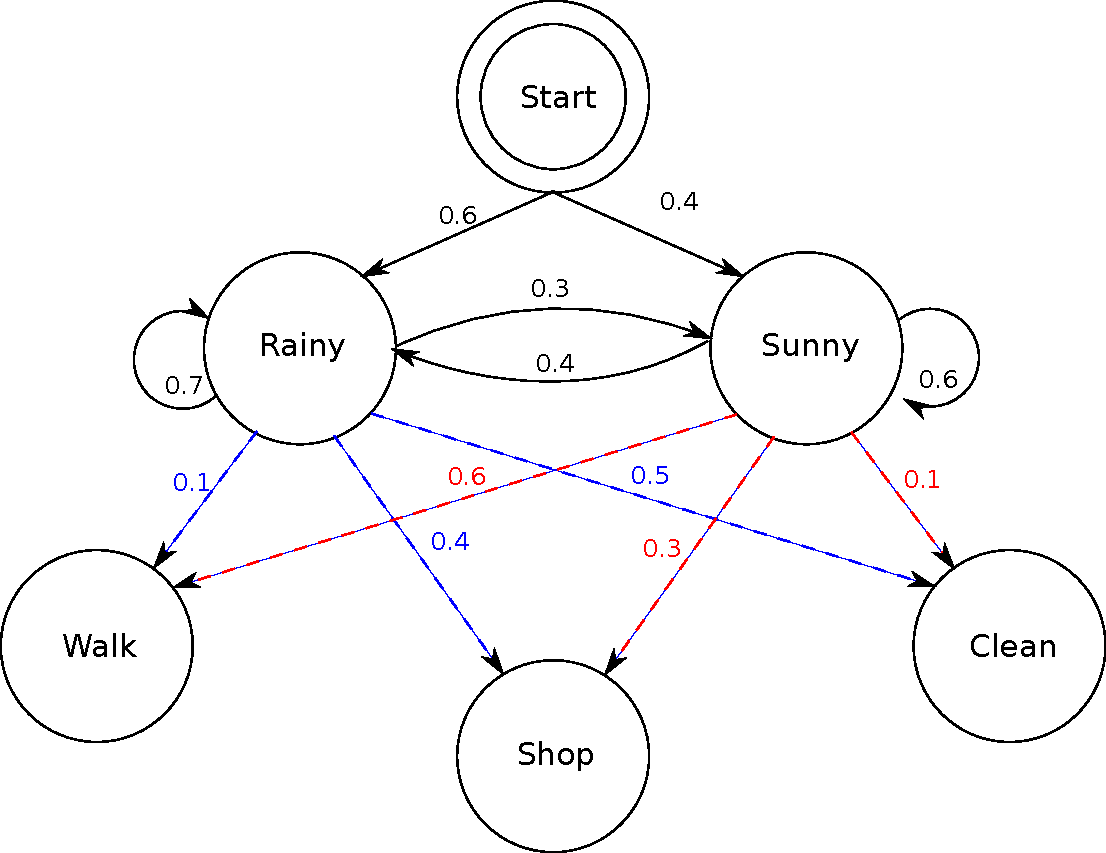
\includegraphics[width=0.6\textwidth]{HMMGraph.pdf}
        %\caption{}
    \end{figure}
    Weather prediction. Sunny and Rainy are hidden states, while the activities are observations.
\end{frame}
%-------------------------------------------------------------------
\begin{frame}{Mathematical Definition}
    A discrete HMM is defined by:
    \begin{itemize}
        \item $N$ hidden states: $S = \{1, 2, ..., N\}$
        \item $M$ possible observations: $V = \{v_1, v_2, ..., v_M\}$
        \item Transition matrix $A = \{a_{ij}\}$ where $a_{ij} = P(X_{t+1} = j | X_t = i)$
        \item Emission matrix $B = \{b_j(k)\}$ where $b_j(k) = P(Y_t = v_k | X_t = j)$
        \item Initial state distribution $\pi = \{\pi_i\}$ where $\pi_i = P(X_1 = i)$
    \end{itemize}
\end{frame}
%----------------------------------------------------------------------------------------------------
\section{Baum-Welch Algorithm}

\begin{frame}{Baum-Welch Algorithm for hidden structure}
    \begin{itemize}
        \item Also known as the Forward-Backward algorithm
        \item Used to find the maximum likelihood estimate of HMM parameters
        \item Given observation sequence $Y = (Y_1=y_1, Y_2=y_2, ..., Y_T=y_T)$
        \item Finds $\theta^* = \argmax_{\theta} P(Y|\theta)$ (or a stationary point)
        \item Parameters $\theta = (A, B, \pi)$ where:
        \begin{itemize}
            \item $A = \{a_{ij}\}$: transition probabilities
            \item $B = \{b_j(y_i)\}$: emission probabilities
            \item $\pi$: initial state distribution
        \end{itemize}
    \end{itemize}
\end{frame}
%----------------------------------------------------------------------------------------------------
\begin{frame}{Baum-Welch as Expectation Maximization}
    \begin{block}{EM Principle}
        \begin{itemize}
            \item Iterative method for finding maximum likelihood estimates
            \item Handles incomplete data by treating hidden states as missing data
            \item Each iteration consists of two steps:
            \begin{itemize}
                \item E-step: Compute expected value of log-likelihood
                \item M-step: Maximize this expectation
            \end{itemize}
        \end{itemize}
    \end{block}
\end{frame}

\begin{frame}{Forward-Backward Procedure}
    \begin{block}{Forward Variable $\alpha_i(t)$}
        Probability of observing sequence $y_1, ..., y_t$ and being in state $i$ at time $t$:
        \[\alpha_i(t) = P(Y_1=y_1, ..., Y_t=y_t, X_t=i | \theta)\]
        \begin{itemize}
            \item Initialization:
            \[\alpha_i(1) = \pi_i b_i(y_1)\]
            \item Recursion:
            \[\alpha_j(t) = b_j(y_t) \sum_{i=1}^N \alpha_i(t-1)a_{ij}\]
            \item Termination:
            \[P(Y|\theta) = \sum_{i=1}^N \alpha_i(T)\]
        \end{itemize}
    \end{block}
\end{frame}

\begin{frame}{Forward-Backward Procedure}
    \begin{block}{Backward Variable $\beta_i(t)$}
        Probability of observing sequence $y_{t+1}, ..., y_T$ given state $i$ at time $t$:
        \[\beta_i(t) = P(Y_{t+1}=y_{t+1}, ..., Y_T=y_T | X_t=i, \theta)\]
        \begin{itemize}
            \item Initialization:
            \[\beta_i(T) = 1\]
            \item Recursion:
            \[\beta_i(t) = \sum_{j=1}^N a_{ij}b_j(y_{t+1})\beta_j(t+1)\]
        \end{itemize}
    \end{block}
\end{frame}

\begin{frame}{E-step: Computing Intermediate Variables}
    \begin{itemize}
        \item Using Bayes' theorem and forward-backward variables:
        \begin{itemize}
            \item Probability of being in state $i$ at time $t$:
            \[\gamma_i(t) = P(X_t=i|Y,\theta) = \frac{\alpha_i(t)\beta_i(t)}{P(Y|\theta)}\]
            \item Probability of transition from $i$ to $j$:
            \[\xi_{ij}(t) = P(X_t=i,X_{t+1}=j|Y,\theta) = \frac{\alpha_i(t)a_{ij}b_j(y_{t+1})\beta_j(t+1)}{P(Y|\theta)}\]
        \end{itemize}
        \item These probabilities are used to compute expected counts:
        \begin{itemize}
            \item Expected time spent in state $i$: $\sum_{t=1}^T \gamma_i(t)$
            \item Expected transitions from $i$ to $j$: $\sum_{t=1}^{T-1} \xi_{ij}(t)$
        \end{itemize}
    \end{itemize}
\end{frame}

\begin{frame}{M-step: Parameter Updates}
    \begin{itemize}
        \item Update parameters to maximize expected log-likelihood:
        \begin{align*}
            \bar{a}_{ij} &= \frac{\sum_{t=1}^{T-1} \xi_{ij}(t)}{\sum_{t=1}^{T-1} \gamma_i(t)} \\
            \bar{b}_j(k) &= \frac{\sum_{t=1}^{T} \gamma_j(t) \cdot \delta(y_t, v_k)}{\sum_{t=1}^{T} \gamma_j(t)} \\
            \bar{\pi}_i &= \gamma_i(1)
        \end{align*}
        \item Each update increases the likelihood:
        \[P(Y|\theta_{new}) \geq P(Y|\theta_{old})\]
    \end{itemize}
\end{frame}

\begin{frame}{Convergence Properties}
    \begin{itemize}
        \item Baum-Welch is guaranteed to converge
        \item However, it may converge to:
        \begin{itemize}
            \item Local maximum (most common)
            \item Saddle point (rare)
            \item Global maximum (not guaranteed)
        \end{itemize}
        \item Quality of solution depends on:
        \begin{itemize}
            \item Initial parameter values
            \item Model structure
            \item Amount of training data
        \end{itemize}
    \end{itemize}
\end{frame}
%----------------------------------------------------------------------------------------------------
\section{Viterbi Algorithm}

\begin{frame}{Viterbi Algorithm for the hidden sequence}
    \begin{itemize}
        \item Dynamic programming algorithm
        \item Finds most likely sequence of hidden states (Viterbi path)
        \item Given observation sequence $Y = (Y_1=y_1, Y_2=y_2, ..., Y_T=y_T)$
        \item Uses two matrices of size $T \times N$:
        \begin{itemize}
            \item $P_{t,s}$: maximum probability of ending at state $s$ at time $t$
            \item $Q_{t,s}$: previous state in the maximum probability path
        \end{itemize}
    \end{itemize}
\end{frame}

\begin{frame}{Viterbi Algorithm Steps}
    \begin{enumerate}
        \item Initialization ($t=0$):
        \[P_{0,s} = \pi_s \cdot b_s(y_0)\]
        \[Q_{0,s} = 0\]
        
        \item Recursion ($t>0$):
        \[P_{t,s} = \max_{r \in S} (P_{t-1,r} \cdot a_{r,s} \cdot b_s(y_t))\]
        \[Q_{t,s} = \argmax_{r \in S} (P_{t-1,r} \cdot a_{r,s})\]
        
        \item Termination:
        \[P^* = \max_{s \in S} P_{T-1,s}\]
        \[X_{T-1}^* = \argmax_{s \in S} P_{T-1,s}\]
        
        \item Path backtracking:
        \[X_t^* = Q_{t+1}(X_{t+1}^*)\]
    \end{enumerate}
\end{frame}
%----------------------------------------------------------------------------------------------------
\begin{frame}{Applications}
    \begin{itemize}
        \item Speech recognition
        \item Natural language processing
        \item Bioinformatics
        \item Financial time series analysis
        \item Weather forecasting
    \end{itemize}
\end{frame}
%----------------------------------------------------------------------------------------------------
\section{Part of speech tagging}
\begin{frame}{NLP: Part-of-speech tagging}
    Brown corpus: 1M tagged words, 15 categories.
    Universal tagset:
    \begin{table}[h]
        \centering
        \begin{tabular}{lll}
            \toprule
            \textbf{Tag} & \textbf{Meaning} & \textbf{Examples} \\
            \midrule
            NOUN & noun & dog, time \\
            VERB & verb & run, is \\
            ADJ & adjective & blue, big \\
            ADV & adverb & quickly, very \\
            PRON & pronoun & I, you, they \\
            DET & determinative & the, a, some \\
            ADP & preposition & in, on, under \\
            NUM & numeral & one, two \\
            CONJ & conjunction & and, but \\
            PRT & particle & up, not \\
            X & unknown & foreign words, typos \\
            . & punctuation & . ! ? , \\
            \bottomrule
        \end{tabular}
    \end{table}
\end{frame}
%----------------------------------------------------------------------------------------------------
\begin{frame}{Supervised vs unsupervised}

Supervised: 
\begin{itemize}
    \item maximum likelihood estimation for training and Viterbi for predicting 
    \item all train dataset ($\approx$ 45 000 sentences), 1.6 sec training, 1.5 min predicting: 73\% test accuracy
    \item random 1000 sentences: 22\%
    \item random 10 000 sentences: 52\%.
    \item random 30 000 sentences: 67\%.
\end{itemize}
Unsupervised:
\begin{itemize}
    \item Baum-Welch takes much more time (105 min)
    \item First 1 000 sentences with tagging, supervised, then all unsupervised. Accuracy = 67\% after 10 iterations.
\end{itemize}
\end{frame}
%----------------------------------------------------------------------------------------------------

\begin{frame}{Additive Smoothing}
    Lidstone smoothing:
    \[
    P_{\text{lidstone}}(w) = \frac{\text{count}(w) + \gamma}{N + \gamma \times V}
    \]

    where:

    \begin{itemize}
    \item $\text{count}(w)$ is the raw count of outcome $w$,
    \item $N = \sum_{x} \text{count}(x)$ is the total number of observations in \texttt{freqdist},
    \item $V = \texttt{bins}$ is the total number of distinct possible outcomes (e.g., vocabulary size).
    \end{itemize}
    Supervised:
    \begin{itemize}
        \item $\gamma = 0.1$ for the estimator 
        \item all train dataset: 95\% test accuracy
    \end{itemize}
    Unsupervised:
    \begin{itemize}
        \item First 1 000 sentences with tagging, supervised, then all unsupervised. Accuracy = 57\% after 10 iterations.
    \end{itemize}
    \end{frame}
%----------------------------------------------------------------------------------------------------
%\section{Stock weather forecasting}
%\begin{frame}{Bull / bear prediction}
% add your predicted transition states
%\end{frame}
% add your plot with red and green

%----------------------------------------------------------------------------------------------------

\begin{frame}{Thank You!}
    \begin{center}
        Questions?
    \end{center}
\end{frame}

\end{document}
